\chapter{MBDyn Adapter and its integration}
\label{cha:adapter}


To prepare an existing simulation code for coupling, preCICE has to be integrated with the solver, using  API described in Section \ref{sec:pc-api} and in Appendix \ref{sec:api-code}. The "glue-code" required for this operation is called \textit{adapter}, as depicted in Figure \ref{fig:adapter-scheme}.


\begin{figure}[htbp!]
	\centering
	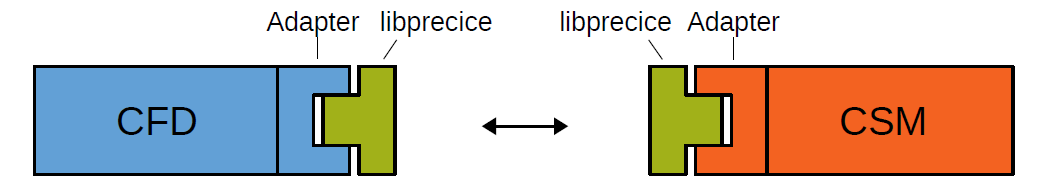
\includegraphics[width=0.92\textwidth]{images/adapter_scheme}
	\caption{Coupling CFD to CSM via preCICE.The existing solver code, the adapter and the linked library are highlighted (image taken from \cite{uekermann2017official}).}
	\label{fig:adapter-scheme}
\end{figure}


\section{Design of the adapter structure}


In order to couple MBDyn with preCICE a C++ adapter has been implemented within the scope of this work. The \textit{adapter} needs to be integrated with both the MBDyn solver and the coupling library. The two connections are distinct but strictly interconnected.
The adapter has the advantage of being completely independent from both the preCICE library and MBDyn. The first connection is achieved via the API given by the library \texttt{libprecice.so}, the second connection exploits the API given by MBDyn through its library \texttt{libmbc.so}.


\section{Structure of the code}

The code for the adapter is available through a public git repository\footnote{\href{https://gitlab.com/Ccaccia73/mbdyn-adapter-test/-/tree/develop}{mbdyn-beam-adapter}}. The code is conceptually divided in two classes, as illustrated in Figure \ref{fig:adapter-classdiag}.

The main class is \texttt{MBDynAdapter}, which implements the functions given by the preCICE interface. It has access to the class \texttt{MBDynConnector} which takes care of all the aspects regarding MBDyn. Attributes, methods and operations of each class are briefly described in the following sections.

\begin{figure}[htbp!]
	\centering
	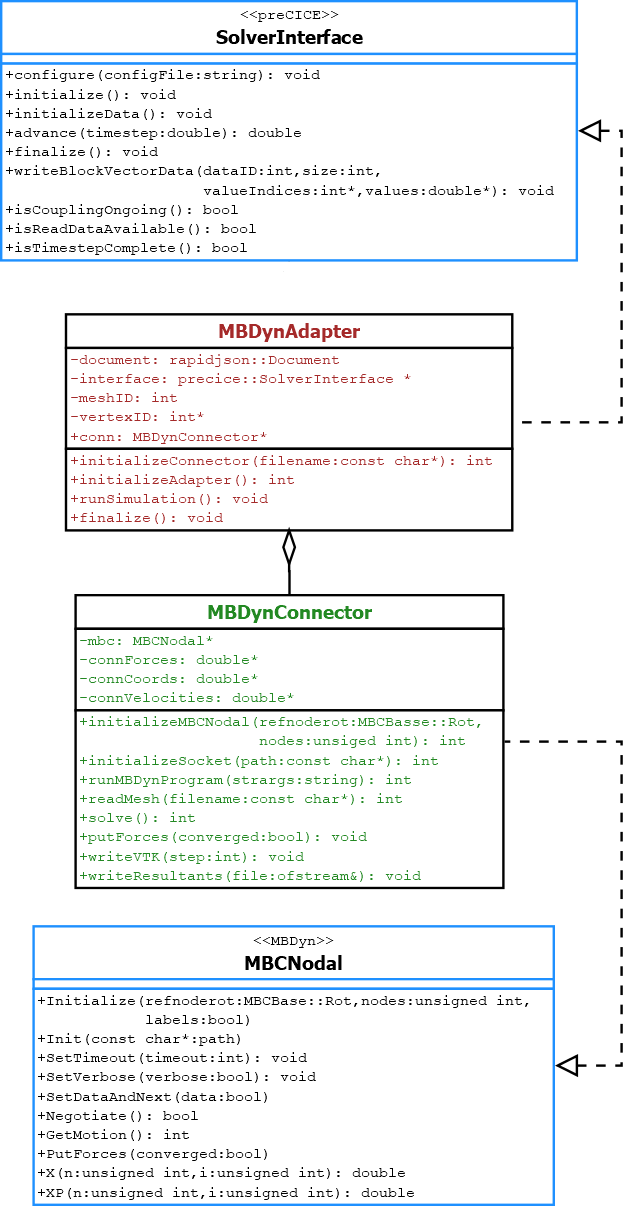
\includegraphics[width=0.76\textwidth]{images/classdiag2}
	\caption{MBDyn adapter class structure}
	\label{fig:adapter-classdiag}
\end{figure}


\subsection{Class MBDynAdapter}
\label{sec:mbdyn-adapter.h}

The file \texttt{MBDynAdapter.h} and its source file \texttt{MBDynAdapter.cpp} implements all the methods required to perform and FSI simulation with MBDyn as the solid solver. The basic steps are:

\begin{enumerate}
	\item prepare the MBDyn solver,
	\item prepare the interface,
	\item provide access to the mesh and initialize the coupling data,
	\item steer the coupled simulation,
	\item finalize the simulation.
\end{enumerate}

\subsubsection{Initialization}

In the initialization phase, the instance of \texttt{MBDynAdapter} gets a \texttt{json} file (see Section \ref{sec:mbdyn-adapter-input}) that contains all the parameters useful for the simulation.
Then it instantiates the \texttt{MBDynConnector} (see Section \ref{sec:mbdyn-connector.h}) which takes care of all the operations concerning MBDyn: in particular starting the simulation the creating an instance of \texttt{MBCNodal} in order to have access to the simulation.

In the next step an instance of \texttt{precice::SolverInterface} is initialized and configured with all the relevant information data:

\begin{itemize}
	\item preCICE configuration file (see Section \ref{sec:pc-config} and Appendix \ref{app:pc-config-file}).
	\item \textit{participant} (i.e. solver) name
	\item information regarding the data to be read and written
\end{itemize} 

The next initialization step concerns the definition of the interface mesh. The data concerning the vertices is stored in the \texttt{MBDynConnector} to be used to plot the output and is passed to the \texttt{SolverInterface} to define the wet surface nodes. The mesh nodes are stored in the same text file that is used by MBDyn to build the \texttt{external structural mapping} information (see Section \ref{sec:mbd-forces}). This means that the MBDyn mapped points coincide with the interface mesh on the structural side (note that it doesn't have to be the same mesh of the fluid side, as preCICE can map non identical meshes, as described in \ref{sec:pc-map}). The suitable size of memory is then initialized to contain the coupling information: mainly \textit{displacements}, to be written on the preCICE interface, and \textit{forces}, to be read from the interface.


\subsubsection{Execution}

The simulation phase of the adapter follows the steps briefly described in Section \ref{sec:pc-api} and in Appendix \ref{app:pc-api}. The most important elements of the codeare  illustrated in listing \ref{lst:adapter-exec}.

The main execution phases include:

\begin{enumerate}
    \item read initial checkpoint (i.e. reload state if previous iteration did not converge) [line 6]
    \item read \textit{forces} from interface (i.e. get the current available fluid solution) [line 10]
    \item copy forces to MBDyn: this step is performed as forces can be scaled by a user specified coefficient during the initial part of the simulation, see Section \ref{sec:mbdyn-adapter-input} [line 14]
    \item make MBDyn connector solve the current simulation time step [lines 16-18]
    \item make MBDyn connector compute force and moment resultants [line 22]
    \item write the \textit{displacements} computed at the current iteration of the current time step to preCICE in order to perform coupling [line 25]
    \item get the interface time step (this would be mandatory in case of different time steps between fuid and solid) [line 28]
    \item check if the current time step is converged [line 31]:
    notify MBDyn on the [lines 35 and 38]. If converged, update time, iterations and write output data (see Section \ref{sec:mbdyn-adapter-output}).
\end{enumerate}

\lstset{language=C++}
\begin{lstlisting}[caption=MBDynAdapter simulation execution,label=lst:adapter-exec]
void MBDynAdapter::runSimulation(){
	// Start coupling:
	while (interface->isCouplingOngoing()){

		if(interface->isActionRequired(cowic)){
			interface->fulfilledAction(cowic);
		}

		// read forces from interface
		interface->readBlockVectorData(forceID, vertexSize, vertexIDs, forces);

		// copy forces to connector with coefficient
		conn->computeForces(forces,coeff);

        // MBDyn solves the current iteration
		if(conn->solve()){
			conn->writeVTK(iteration);
			break;
		}
        
        // compute force and moment resultants on the structure
		conn->computeResultants(true, root);

		// write data to interface
		interface->writeBlockVectorData(displID, vertexSize, vertexIDs, displacements);

		// advance time step
		precice_dt = interface->advance(precice_dt);

		// Checkpoint
		if(interface->isActionRequired(coric)){
			// timestep not converged
			interface->fulfilledAction(coric);
			// tell MBDyn that time step not converged
			conn->putForces(false);
		}else{
			// timestep converged
			conn->putForces(true);
			iteration++;
			t += precice_dt;
			conn->writeVTK(iteration);
		}
	}
}

\end{lstlisting}


\subsubsection{Finalization}

In the finalization phase all the object used during the simulation are closed and memory released.

\subsection{Class MBDynConnector}
\label{sec:mbdyn-connector.h}

The class \texttt{MBDynConnector} takes care of all the operations related to MBDyn and the structural side of the simulation. 

\subsubsection{Initialization}

The instance of \texttt{MBDynConnector} is initialized within the \texttt{MBDynAdapter} and some different tasks are performed in this phase.

The first task is to read the mesh of interface points. The mesh file location is passed through the input file: to avoid too much duplication, it is the same file used by MBDyn to build the mapping matrix before the simulation (see Section \ref{sec:mbd-forces}). The mesh file contains information concerning the interface points and the connectivity. The $(x,y,z)$ coordinates are passed to preCICE to build the structural part of the interface mesh. The same points, together with the connectivity, are stored in the \texttt{MBDynConnector} and are used to write the output in \textit{VTK} format during the simulation (see Section \ref{sec:mbdyn-adapter-output}).

The following task consists in starting MBDyn. The input file location is passed through the input file and a separated process is spawned with the parameters required to run an MBDyn program. Upon a correct initialization, the MBDyn simulations hangs waiting for an external connection (i.e. the \texttt{external structural mapping}).

Finally, an instance of \texttt{MBCNodal} is created to take care of the communication with MBDyn: a socket is opened and the communication is initialized. 


\subsubsection{Execution}

During the execution phase, \texttt{MBDynConnector} steers the simulation on the MBDyn side. Some of the actions have been already introduced in listing \ref{lst:adapter-exec}:

\begin{itemize}
    \item send \textit{forces} to the \texttt{external structural mapping} points
    \item perform the simulation step
    \item retrieve \textit{displacements}
    \item inform MBDyn that the time step has converged or not
\end{itemize}

If the time step has converged and at a user defined interval, the simulation data are saved.


\section{Input parameters}
\label{sec:mbdyn-adapter-input}



input: json config file

- simulation parameters

\section{Output results}
\label{sec:mbdyn-adapter-output}

output: VTK and resultants
